\documentclass[12pt]{article}

% Any percent sign marks a comment to the end of the line

% Every latex document starts with a documentclass declaration like this
% The option dvips allows for graphics, 12pt is the font size, and article
%   is the style

\usepackage[pdftex]{graphicx}
\usepackage{url}
\usepackage{xcolor}
\usepackage{sectsty}

\subsectionfont{\color{blue}}  % sets colour of chapters
\sectionfont{\color{cyan}}

% These are additional packages for "pdflatex", graphics, and to include
% hyperlinks inside a document.

\setlength{\oddsidemargin}{0.25in}
\setlength{\textwidth}{6.5in}
\setlength{\topmargin}{0in}
\setlength{\textheight}{8.5in}

% These force using more of the margins that is the default style

\begin{document}

% Everything after this becomes content
% Replace the text between curly brackets with your own
\begin{titlepage}
\title{{\Huge Project Scope}\\
{\huge \color{cyan}Project Name: Distributed Timesheet}}
\author{{\huge{\color{blue}Customer Name: ACME}}\\
	\\{\small Requirements Engineers:}
\\Robert Pate\\robert.pate@gmail.com\\\\Neel Shah\\neel.shah.528@gmail.com\\\\Adam Whipple\\awhipple@utexas.edu\\\\Gregory Williams\\grw300@gmail.com}
\date{\today}

% You can leave out "date" and it will be added automatically for today
% You can change the "\today" date to any text you like


\maketitle
\vfill
\end{titlepage}
% This command causes the title to be created in the document

\section{Product Overview}

The Web-based Timesheet System is intended to allow a globally distributed workforce to record details of their time expenditures working for a variety of clients as well as non-project time codes.  Users can either click “start/stop” timers throughout the day or simply add time on a weekly timesheet.

Managers have access to simple reports displaying how much time employees have tracked against tasks and can approve or send back to the employee for edits.

The system will also support superusers who can add or subtract client codes from individual workers’ timesheets, edit timesheets directly, send them back to the worker for editing, or export the time data into a bookkeeping / invoicing system such as Quickbooks (.iif), Peachtree, ADP, and common formats such as excel, XML, and CSV. The system will have basic reporting capabilities for the first release.

\section{Packaging}

Ultimately, this system will be part of a suite of products for B2B SaaS packaging.  Therefore, the system needs to be easily implemented, highly maintainable, work on a variety of machines: web (Firefox, Chrome, IE?/Edge, Safari).  The system should also have a web portal where customers can register and purchase a plan.  For the first release, the product will be free.

\section{Future Development}

A later version of this system could also address timekeeping requirements for government contractors in accordance with DCAA (Defense Contract Audit Agency - \url{http://www.dcaa.mil/DCAAM_7641.90.pdf}) however, this is out of scope for the first release.  Also intended for later release is a Desktop (macOS, Windows) application and a mobile application Mobile (Android, iOS).  As features are added in later releases, additional plan levels and costs will be added to the web portal.

\section{Competitors}

Top 3 competitors include:\\
Yast - \url{http://www.yast.com/}\\
Harvest - \url{https://www.getharvest.com/}\\
Toggl - \url{https://www.toggl.com/}

\section{Stakeholders}

In order to have robust requirements, we need to determine who the stakeholders are and prioritize them for interviews. We will not have time to interview all stakeholders, so it’s helpful to categorize them into groups that should have similar roles and requirements. Many of these categories are common across various systems. Listing them will help ensure we have stakeholder coverage for them.

\subsection{Domain Viewpoint Hierarchy}

\begin{center}
	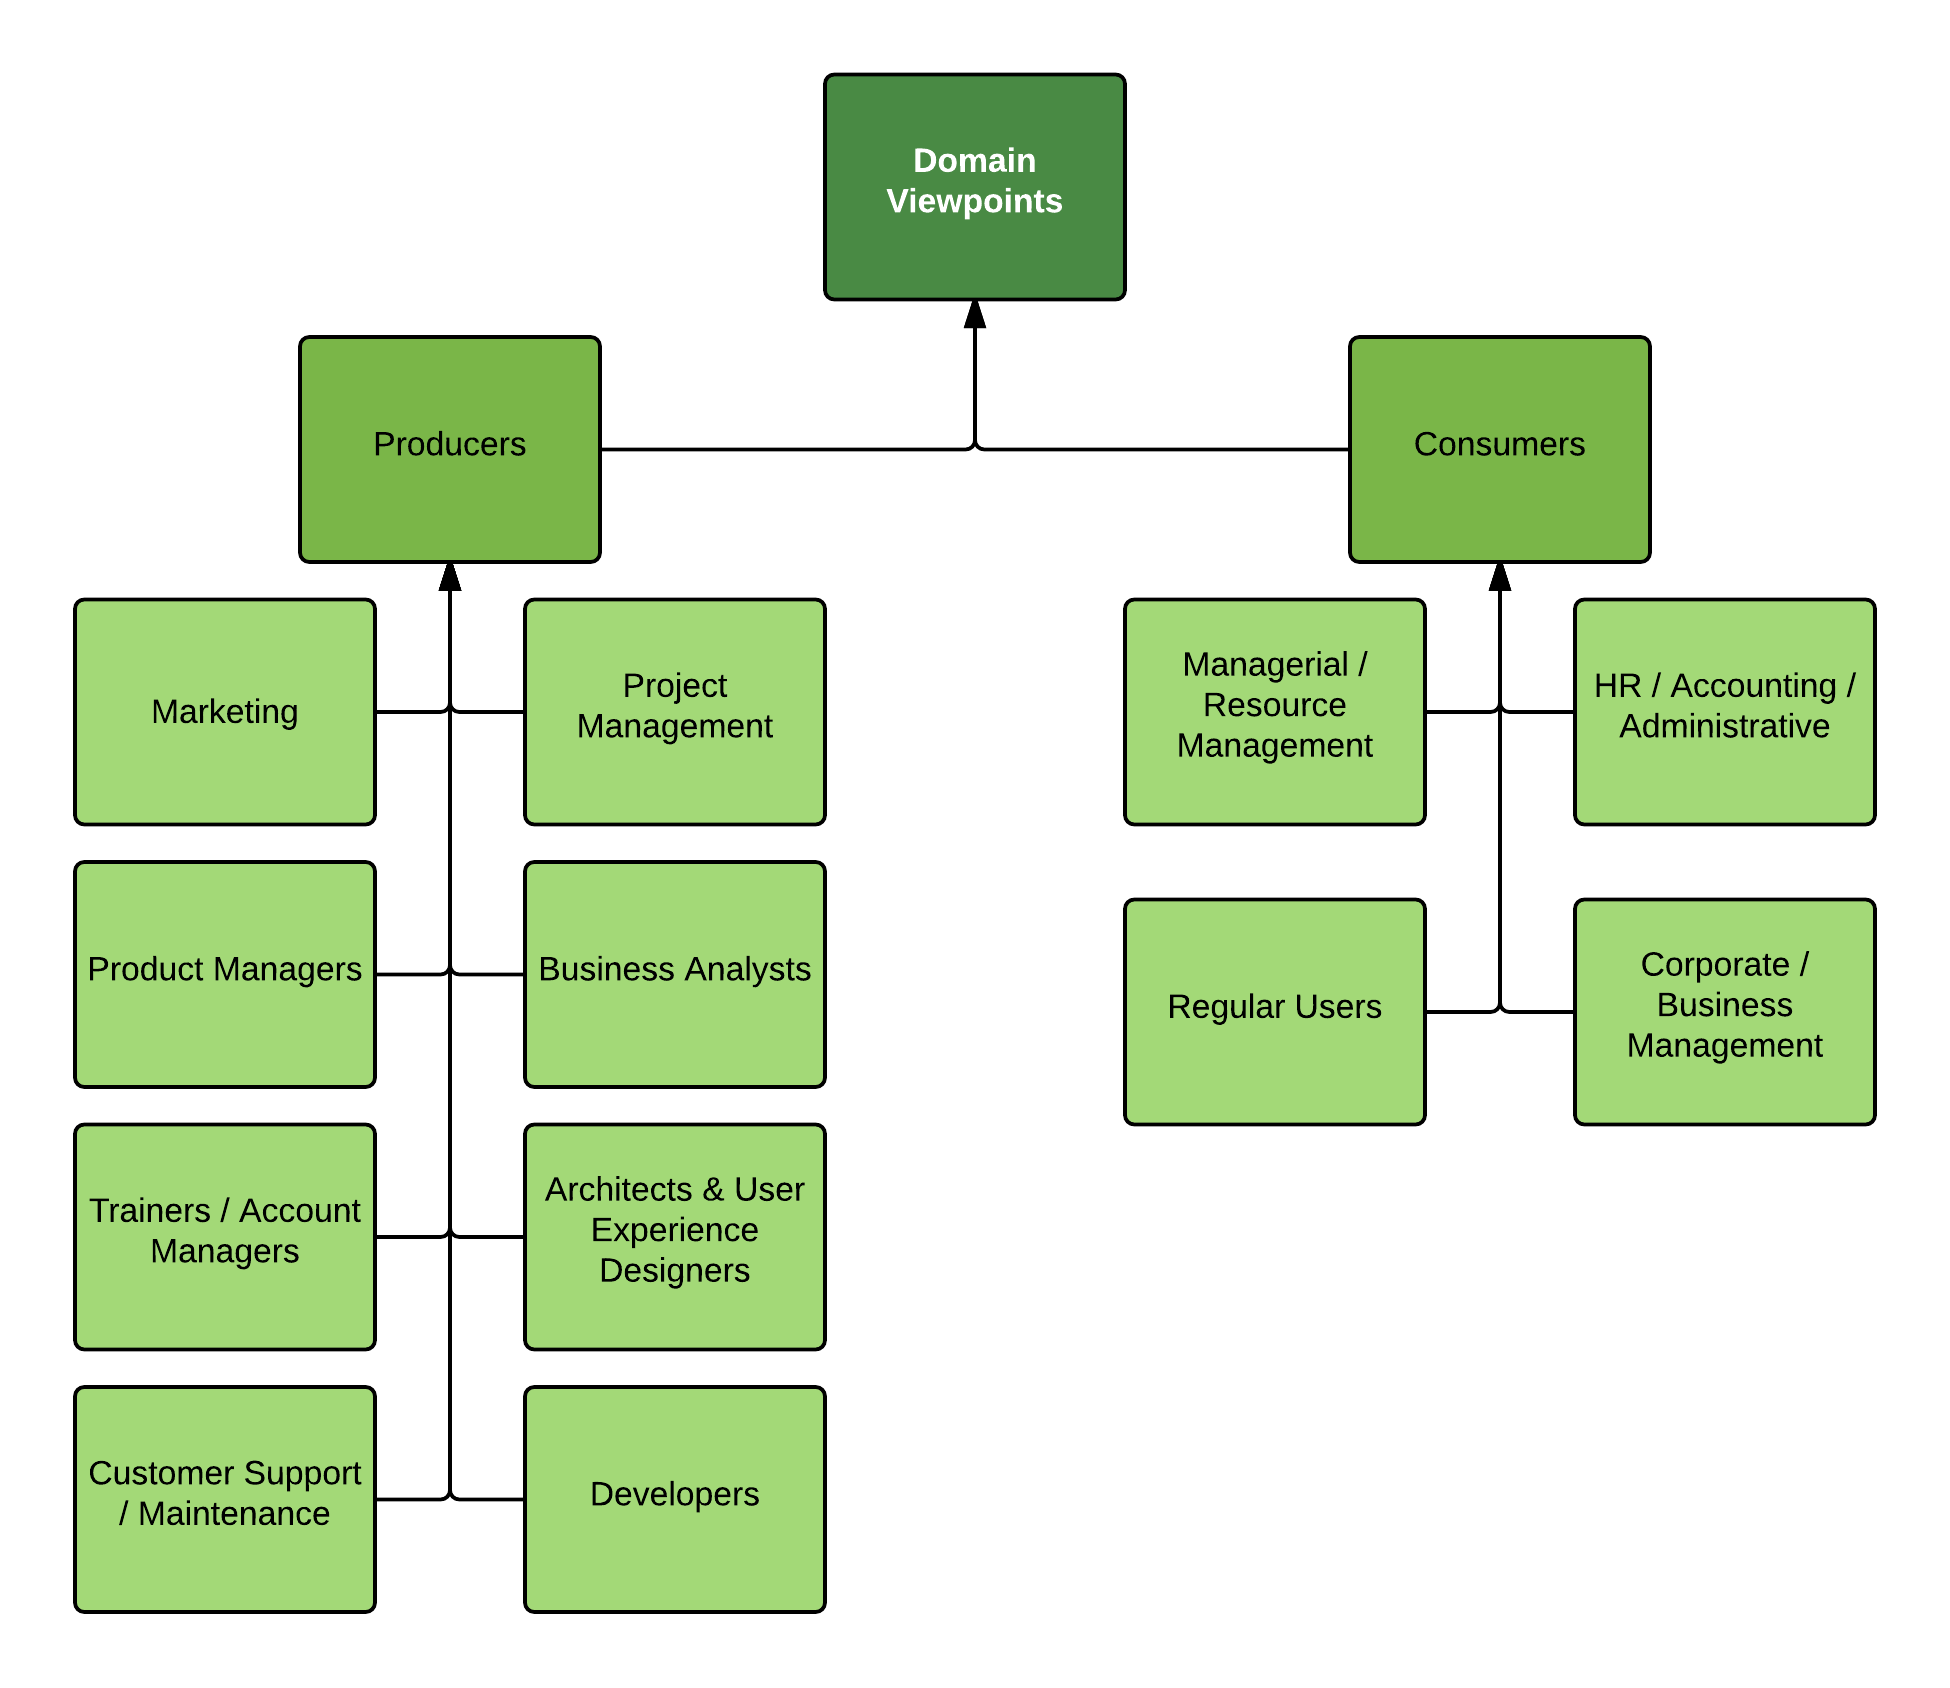
\includegraphics{Graphs/DomainView}
\end{center}
Consumers share similar requirements for system access and how often they’ll use the system. What differs between the consumers is the primary use case for each role. Management will be reviewing the timesheets of their direct reports, HR will be orchestrating payment, regular users will be logging time, and Corporate will be defining the high level goals. Management, HR, and Regular users are included in the stakeholder interviews. Corporate’s goals are covered by the Product Manager.

Producers make up the team developing the system. Some may end up being regular users once the system is launched, but their focus will be on non-functional requirements. The Product Manager and a developer are included in the stakeholder interviews.

\subsection{Organization Viewpoint Hierarchy}

\begin{center}
	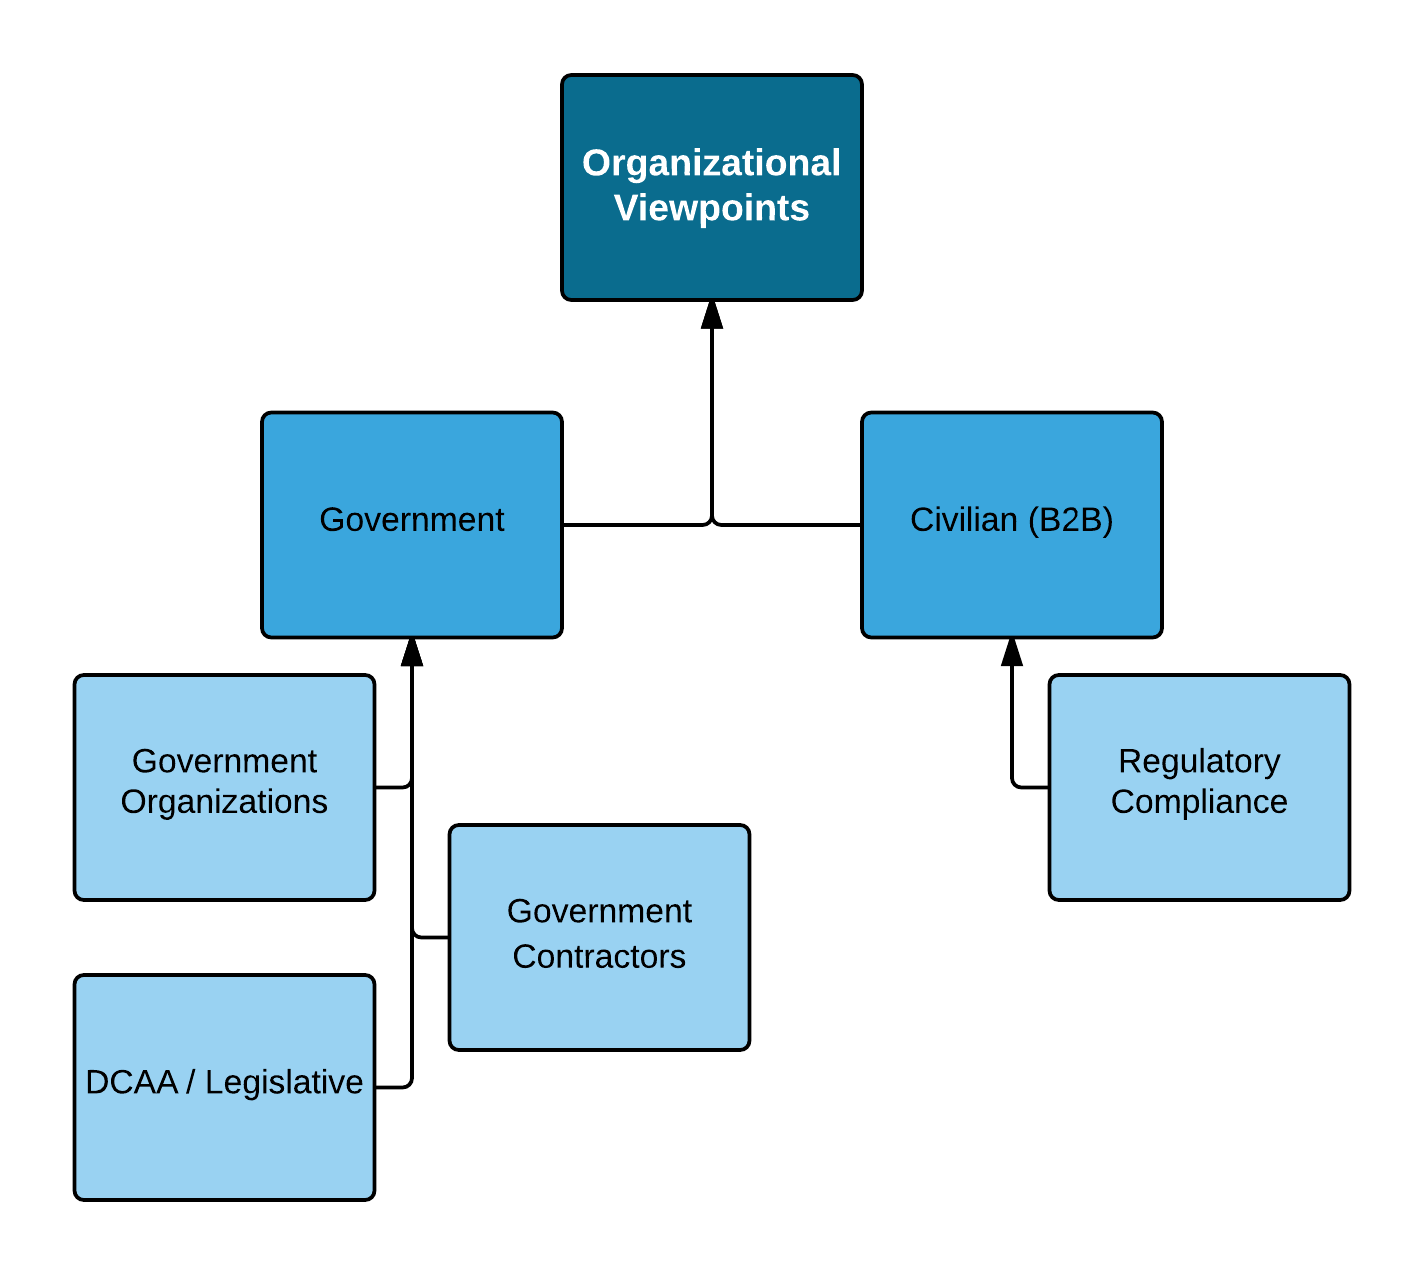
\includegraphics{Graphs/OrgView}
\end{center}

\subsection{Description of Stakeholders}

\subsubsection{Marketing / Product Manager}
The Marketing / Product Manager is required to understand the product domain space from a business perspective and to develop financial, functional, and nonfunctional metrics for the product.  This individual is ultimately responsible for the success or failure of the product over its lifecycle.

\subsubsection{Human Resources / Accounting  SME}
The HR/Accounting Subject Matter Expert (SME) is an individual who interacts with timekeeping and other downstream systems in the payroll/invoicing process.  This individual will represent the requirements of the HR/Accounting superuser role.

\subsubsection{Manager SME}
The Manager SME is an individual who interacts with timekeeping on a managerial level, responsible for tracking and approving/disapproving time entered by employees.  This individual will represent requirements of the manager role.


\subsubsection{User}
The User SME is an individual who interacts with timekeeping systems on a regular basis: entering / recording time for various time codes.

\subsubsection{Project Manager / SCRUM Master}
Manage the overall development process: guide development team, assist product manager, manage project communication, etc.  This role may be responsible for understanding or uncovering project requirements and constraints as well as Legacy system usage and integration.

\subsubsection{The Developer}
The Developer represents the employees that will provide the final implementation of the product. To do this, the Developer will need to have a complete understanding of the functional and nonfunctional requirements.

\subsubsection{Corporate}
The Corporate stakeholder group represents the companies that will purchase the final implementation of the product. They drive the primary goals of the system and communicate them to Marketing and the Product Manager. They won’t use the system, but they to make sure it has a good return on the investment.


\subsection{Priority Stakeholders}
\begin{itemize}

\item Product Manager - This individual is the project sponsor and is ultimately responsible for the success or failure of the product.  This role is required to represent the needs of both the end user as well as the business.\\

\item Human Resources / Accounting SME - This user represents the customer most likely to drive purchase and integration of this product within the client organization.  This role is key in turning data entered into the system by other users into actionable payroll, invoicing, and reporting data.\\

\item Manager - While this role occupies a User role, there is additional functionality that this user will employ - approval / denial, and reporting -  therefore, this user’s needs (beyond the regular user) should be considered. Furthermore, this user will be key in adopting and integrating this platform (Organizational Change Management.)\\

\item User - This role represents the largest customer group intended to use the system.  While this role is not key in integrating the system with other processes such as accounting, payroll, etc, this role is key in adoption of this system.  This role will interact with the system either continually throughout the day or at least on a daily basis.\\

\item Developer - This stakeholder is not intended as an end user, though could be considered in a maintenance role.  While this stakeholders needs should be taken into account, they should not trump the needs of the paying customers.
\end{itemize}


\section{Operational Reference Model}

The Operational Reference Model will set boundaries on expected capabilities. Setting these boundaries is beneficial so that all stakeholders are on common ground when it comes to describing Project Scope and allows for definition and focus on the Project itself. The ORM is a useful tool for describing the boundary conditions because it is graphical, concise, and encapsulates higher level functional categories.

\subsection{ORM Diagram}

\begin{center}
	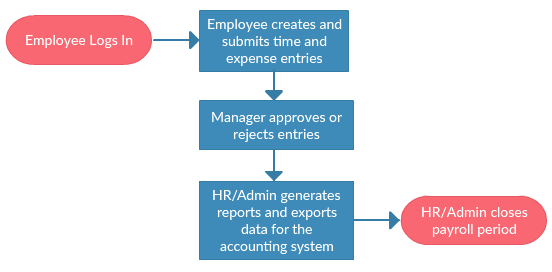
\includegraphics[scale=.85]{Graphs/ORM}
\end{center}

\subsection{Description}

The operational model is triggered when “Employee Logs In”. This initiates interaction with the System. Without this event, no other functionality of the System is required. The first operation continues the Employee interaction and allows that role to “Create and Submit Time Entries”. After the entries are submitted, the Manager begins interacting with the System and “Approves or Rejects Entries”.

Finally, the HR/Admin role is involved and “Generates Reports and Exports Data for the Accounting System”. This delineates the functionality of the System from accounting functionality. Termination occurs when “HR/Admin Closes Payroll Period”, preventing interaction for the period in question and allowing the operational flow to occur once more.

\section{Key Scenarios}
Key scenarios loosely track the type of requirements and provide examples of the identified must-do's of the system. They represent the pieces of functionality that must be accommodated in order to create the system that will be defined by the requirements.

\subsection{ Employee logs into system}
\begin{itemize}
\item Scenario Description:
An employee will have a login account that is uniquely defined with a company email address. After entering a company-specific web address into one of the supported browsers (e.g. https://www.TimeSystem.com/Some.Company) an emplyee will be prometed to enter their credentials that have been populated by the customer (no employee should create an account). If this is their first time logging into the system, they will be prompted to change their password. A successful login will present the “Project Time Entry” screen and employees can then begin logging their time.
\item Coverage of ORM:
\begin{itemize}
\item Employee creates and submits time entries
\end{itemize}
\end{itemize}

\subsection{ Manager logs into system}
\begin{itemize}
\item Scenario Description: Managers will go through the same first-time login experience as employees. On successful login, managers will have an “Project Time Entry” option, a “Create Project” option, and a “Approve Time Entry” option. The Approve Time Entry option will display all the project that their employees have charged time to for that time period.
\item Coverage of ORM:
\begin{itemize}
\item Employee creates and submits time entries
\item Manager approves or rejects entries
\end{itemize}
\end{itemize}

\subsection{ Employee creates time entries}
\begin{itemize}
\item Scenario Description: Employees will have predefined projects that they can select from; they will also have templates (e.g. “Predefined” by a manager, “Last-Submission” that creates all time entries that were submitted for the last time period, or “Custom”) for the employee to select. Each project will have a field for recording the billable hours. There will be “Clear”, “Cancel”, and “Submit” options.
\item Coverage of ORM:
\begin{itemize}
\item Employee creates and submits time entries
\end{itemize}
\end{itemize}

\subsection{ Manager Creates Predefined Project}
\begin{itemize}
\item Scenario Description: After selecting the “Create Project” option on the login screen, managers will be presented with an HTML form that asks for “Project Name”, “Project Identifier”, “Project Customer”, and “Project Billable Price”; only the “Projectr Identifier” will be required. There will also be an option for “Custom Project Field” that will present an additional form entry: any “Custom Project Fields” will be stored in serializable format for use when employees use “Predefined” projects. There will be “Clear”, “Cancel”, and “Submit” options.
Coverage of ORM:
\begin{itemize}
\item Employee creates and submits time entries
\item Manager approves or rejects entries
\item Admin generates reports and exports data for the accounting system
\end{itemize}
\end{itemize}

\subsection{ Employee Submits Time Entry}
\begin{itemize}
\item Scenario Description: After clicking the “Submit” button for the time entries, the employee will be presented with a static, uncluttered, view of their time entries. The employee will be prompted to “Confirm” or “Cancel” the time entry submission.
\item Coverage of ORM:
\begin{itemize}
\item Employee creates and submits time entries
\end{itemize}
\end{itemize}

\subsection{ Manager is Notified of Time Entry Submittion}
\begin{itemize}
\item Scenario Description: When an employee submits an time entry, the manager will be emailed about the successful employee submission. There will be a link in the email that will take the manager to their personal system web page for login where they can view all submitted time entries or, if they are already logged in the current browser session, directly to that employee’s submission. Besides the employee entry, there will be calculated “Billable hours” and “Billable cost” entries that provide a quick glance at those metrics for custom projects. If the employee submitted time entries that were not a part of the predefined projects with cost metadata, the estimates will be colored red, if all time entries have costs defined, the estimates will be colored green. There will be “Accept”, “Reject”, and “Cancel” options.
\item Coverage of ORM:
\begin{itemize}
\item Employee creates and submits time entries
\item Manager approves or rejects entries
\end{itemize}
\end{itemize}

\subsection{ Manager Accepts Time Entry}
\begin{itemize}
\item Scenario Description: The manager is presented with a “Confirm” or “Cancel” prompt. After confirmation, the time entry will be removed from the manager’s login page. The employee is notified by email that their time entry submission was accepted.
\item Coverage of ORM:
\begin{itemize}
\item Manager approves or rejects entries
\end{itemize}
\end{itemize}

\subsection{ Manager Rejects Time Entry}
\begin{itemize}
\item Scenario Description: The manager is presented with a “Confirm” or “Cancel” prompt. After rejection, the time entry will be removed from the manager’s login page. The employee is notified by email that their time entry was rejected and provided a link that will populate their time entry submission for with the information that was rejected. If the employee attempts to submit again without changes, they will be prompted with an additional dialog that warns them that no changes were made. They will be able to go back and add changes, or prompt the system to continue with the submission.
\item Coverage of ORM:
\begin{itemize}
\item Employee creates and submits time entries
\item Manager approves or rejects
\end{itemize}
\end{itemize}

\subsection{ Admin Receives a Batch of Time Entries}
\begin{itemize}
\item Scenario Description:
Once managers approve of all of their employee’s time entries, they will have an option of submitting a report to the admins. This will clear all the time reports from the managers web page, and notify the admin’s by email that an time report collection has been submitted.
\item Coverage of ORM:
\begin{itemize}
\item Manager approves or rejects entries\\
\item Admin generates reports and exports data for the accounting system
\end{itemize}
\end{itemize}

\subsection{ Admin Creates Report and Export}
\begin{itemize}
\item Scenario Description:
Once the admins have received a batch of time entries, they will be able to select an export format that the system supports and generate the export. They will also be able to run pivots against the submitted entries that select for the fields provided by the employees and approved by the managers, and export that information. The admins will have the option to save their export settings as a preset, and they will be able to save many presets. For example, an admin may run a pivot to generate the total billable hours to a specific customer, and then export that information as a top row above the rest of the custom information in a CSV format. When the admin is prompted for submission, they will have a listbox of their saved presets next to an “Apply” option that will perform the correct data manipulation and exporting. There will be a “Archive” button that will remove the report data from their immediate web page, but this submission will be saved for a period before deletion.
\item Coverage of ORM:
\begin{itemize}
\item Manager approves or rejects entries\\
\item Admin generates reports and exports data for the accounting system
\end{itemize}
\end{itemize}


\end{document}